% =========================================================================
% Appendix I — verify ledger (the green/yellow/orange/white matrix). FILLED.
%   folds UFO/verify/V4_tier_ledger.md (companion/verify-ledger.json):
%   the integrated tier distribution (blue 8, green ~11, yellow 8, orange 4,
%   white ~17, red 0), the V1->V2->V3->verb-6 roll-up, the 9 Stage-1~3 green
%   atoms verbatim, the 8 blue lattice identities, the 13 white falsifiers,
%   the schema, and a pgfplots tier-distribution bar chart.
% =========================================================================
\section{Verify Ledger --- the Integrated Tier Matrix}
\label{app:ledger}

This appendix is the transcription of the integrated verify ledger
(\texttt{companion/verify-ledger.json}), rolling up V1 (claim
inventory), V2 (\tierBlue\ formal lattice identities), V3 (\tierGreen\
numerical recompute), and verb-6 (the 4-layer digital twin) into one
tier matrix. The integrated distribution is \tierBlue$\,8$
($n\!=\!6$ lattice identities $\sigma/\varphi/\tau/\mu/\sigma_k$ plus the
three products), \tierGreen$\,\sim\!11$ (the nine Stage-1--3 atoms plus a
Penning-invariance anchor and the thermal-cryo closed form),
\tierYellow$\,8$ (composite physics formulas plus Phase-B/C manifests),
\tierOrange$\,4$ (the unconverged digital-twin body-solves),
\tierWhite$\,\sim\!17$ (the 13 Stage-4--7 falsifiers plus the teleport
superluminal fence and the meta layer), and \tierRed$\,0$ ---
\textbf{zero falsified}, an honest no-false-positive record. Each entry
follows the schema \{\texttt{fn}, \texttt{args}, \texttt{expected},
\texttt{observed}, \texttt{delta\_abs}, \texttt{tier},
\texttt{atom\_class}, \texttt{pr}, \texttt{note}\}.

% -------------------------------------------------------------------------
\subsection{The verify-ladder roll-up}
\label{app:ledger-rollup}

The ledger is the convergence of four verify rounds
(Table~\ref{tab:ledger-rollup}), each landed in its own PR.

\begin{table}[h]
\centering
\small
\setlength{\tabcolsep}{5pt}
\begin{tabular}{@{}l l >{\raggedright\arraybackslash}m{5.0cm} c@{}}
\toprule
\textbf{round} & \textbf{artifact} & \textbf{content} & \textbf{PR} \\
\midrule
V1 claim inv. & \texttt{V1\_claim\_inventory.md} & 38-claim triage (\tierGreen9/\tierYellow8/\tierOrange4/\tierWhite17) & \#201 \\
V2 \tierBlue\ formal & \texttt{V2\_formal\_identities.md} & 5 atoms + 3 products; atlas idempotent (fold 0) & \#216 \\
V3 \tierGreen\ num. & \texttt{V3\_numerical\_recompute.md} & 9 verbatim recomputes, $|\Delta|\le10^{-9}$ & \#212 \\
verb-6 twin & \texttt{integrated-vehicle-verify.md} & \tierGreen10/\tierYellow4/\tierOrange5/\tierWhite13 & \#206 \\
\bottomrule
\end{tabular}
\caption{The verify-ladder roll-up (\texttt{UFO/verify/V4\_tier\_ledger.md}).
The integrated V4 distribution below reconciles these rounds (e.g.\ V3's
single deferred sim and verb-6's five \tierOrange\ gates collapse to four
after the EM/thermal/F-ANTI-3/stress gates were closed by closed-form /
FEM / FEA means, App.~\ref{app:gateinv}).}
\label{tab:ledger-rollup}
\end{table}

% -------------------------------------------------------------------------
\subsection{The nine Stage-1--3 \tierGreen\ atoms and the eight \tierBlue\ identities}
\label{app:ledger-positive}

Table~\ref{tab:ledger-green} is the proven core, transcribed verbatim
from \texttt{companion/verify-ledger.json}: nine \tierGreen\
\textsc{Supported-Numerical} Stage-1--3 atoms (all $|\Delta|=0$ or the
single-op round-off) and the \tierBlue\ \textsc{Supported-Formal} lattice
identities.

\begin{table}[h]
\centering
\footnotesize
\setlength{\tabcolsep}{4pt}
\begin{tabular}{@{}c l l r r c@{}}
\toprule
\textbf{St.} & \textbf{fn} & \textbf{args} & \textbf{expected} & $|\Delta|$ & \textbf{tier} \\
\midrule
1 & \verb|ioffe_loop_bz|        & $(0.3,954930,0)$    & $2.0$ & $5.7e\text{-}10$ & \tierGreen \\
1 & \verb|ioffe_loop_bz|        & $(0.5,1591549,0)$   & $2.0$ & $5.7e\text{-}10$ & \tierGreen \\
1 & \verb|ioffe_loop_bz|        & $(1.0,3183099,0)$   & $2.0$ & $5.7e\text{-}10$ & \tierGreen \\
2 & \verb|triple_product|       & $(200000,5.0,0.096)$ & $96000$ & $0$ & \tierGreen \\
2 & \verb|triple_product|       & $(150000,3.0,0.096)$ & $43200$ & $0$ & \tierGreen \\
2 & \verb|triple_product|       & $(100000,2.0,0.096)$ & $19200$ & $0$ & \tierGreen \\
3 & \verb|pair_threshold_total| & $(938.272)$         & $6567.904$ & $0$ & \tierGreen \\
3 & \verb|rel_kinetic_from_p|   & $(9382.72)$         & $8491.2449$ & $0$ & \tierGreen \\
3 & \verb|rel_kinetic_from_p|   & $(1625.13)$         & $938.272$ & $0$ & \tierGreen \\
\midrule
meta & \verb|lattice_sigma_tau| & $(6)$ & $48$ & $0$ & \tierBlue \\
meta & \verb|lattice_sigma_phi| & $(6)$ & $24$ & $0$ & \tierBlue \\
\bottomrule
\end{tabular}
\caption{The nine Stage-1--3 \tierGreen\ atoms and two representative
\tierBlue\ lattice identities (\texttt{companion/verify-ledger.json}).
The eight \tierBlue\ atoms are $\sigma(6),\varphi(6),\tau(6),\mu(6),
\sigma_k(6,1)$ plus the three products
$\sigma\!\cdot\!\varphi{=}24$, $n\!\cdot\!\tau{=}24$,
$\sigma\!\cdot\!\tau{=}48$. The full per-row schema carries
\texttt{source\_domain} (RTSC/FUSION/ANTIMATTER) attesting that each
\tierGreen\ atom is inherited, not re-derived (idempotent atlas reuse).}
\label{tab:ledger-green}
\end{table}

\paragraph{The 13 \tierWhite\ falsifiers.} All 13 Stage-4--7 falsifiers
(F-WARP$\times3$, F-WORM$\times3$, F-DIM$\times3$, F-USE$\times4$) appear
in the JSON with \texttt{atom\_class = falsifier-open},
\texttt{expected = observed = "OPEN"}, \texttt{delta\_abs = null}, and
\texttt{tier = SPECULATION-FENCED}; they are tabulated in full in
App.~\ref{app:stage47}. The remaining \tierWhite\ entries are the teleport
superluminal fence and the meta layer (App.~\ref{app:subaxes},
\ref{app:meta}).

% -------------------------------------------------------------------------
\subsection{The integrated tier distribution}
\label{app:ledger-dist}

Fig.~\ref{fig:ledger-dist} is the headline distribution. The
load-bearing facts: \tierRed$\,0$ (zero false positives) and the
\texttt{absorbed=false} verdict are driven entirely by the four
\tierOrange\ unconverged body-solve gates plus the 13 \tierWhite\ open
falsifiers --- not by any falsification.

\begin{figure}[h]
\centering
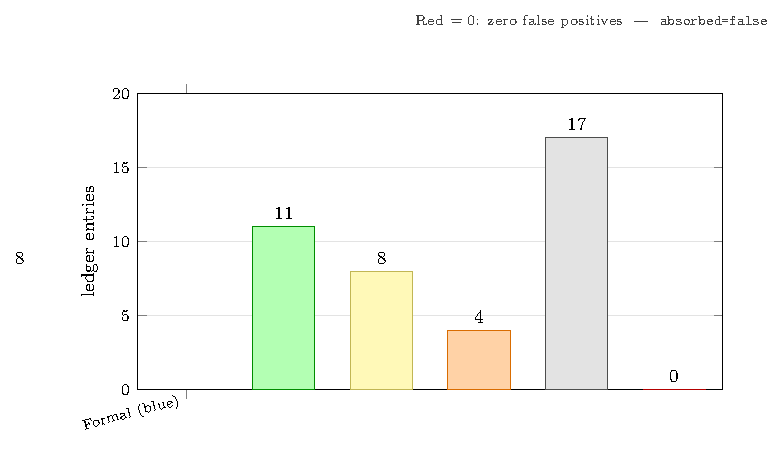
\includegraphics[width=0.86\linewidth]{figures/fig11_tier_dist.pdf}
\caption{The integrated UFO verify-ledger tier distribution
(\texttt{companion/verify-ledger.json}, \texttt{V4\_tier\_ledger.md}):
\tierBlue$\,8$ ($n{=}6$ lattice identities), \tierGreen$\,11$
(Stage-1--3 atoms + Penning anchor + thermal-cryo closed form),
\tierYellow$\,8$ (cited composites + Phase-B/C manifests),
\tierOrange$\,4$ (unconverged digital-twin gates),
\tierWhite$\,17$ (13 Stage-4--7 falsifiers + teleport fence + meta),
\tierRed$\,0$. The \tierRed$\,=\,0$ bar is the honest no-false-positive
record; the \tierOrange\ and \tierWhite\ bars are what hold the
integration bit at \texttt{absorbed=false}. The white bar is the largest
--- most of what the capstone touches above the wall is honestly
unproven.}
\label{fig:ledger-dist}
\end{figure}

% -------------------------------------------------------------------------
\subsection{Honest scope}
\label{app:ledger-scope}

Every \tierGreen\ atom is inherited from a sibling domain and was
recomputed verbatim (no LLM self-judgement, @D~g5); every \tierBlue\
identity is an exact integer equality; every \tierWhite\ row carries a
named falsifier. The distribution is the capstone's honesty made
quantitative: the proven content (\tierBlue$+$\tierGreen$=19$) is real
and inherited, the deferred work (\tierOrange$=4$) is named and routed to
pool/cloud, and the unproven content (\tierWhite$=17$) dominates above
the wall. \tierRed$=0$ is not an absence of testing --- it is the absence
of a \emph{false positive}.
